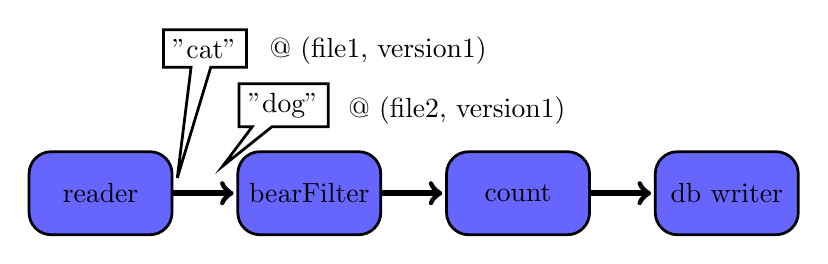
\begin{tikzpicture}[node distance = 0.8cm, auto]
\usetikzlibrary{shapes,arrows}
\usetikzlibrary{positioning}

\tikzstyle{operator} = [rectangle, draw, fill=blue!60, text width=4.5em, text centered, rounded corners = 8pt, minimum height=30pt, line width=1pt]
\tikzstyle{callout} = [draw, rectangle callout, callout relative pointer={#1}, line width=1pt]

    \node [operator] at (0, 0) (reader) {reader};
    \node [operator, right = of reader] (filter) {bearFilter};
    \node [operator, right = of filter] (count) {count};
    \node [operator, right = of count] (writer) {db writer};

    \draw [thick,->,shorten >=1pt, line width=2pt] (reader) -- (filter) 
       node[callout={(-0.3,-40pt)}, midway,above = 45pt] {"cat"} node[midway,above= 45pt, shift={(2.2,-0.1)}] {@ (file1, version1)}
       node[callout={(-0.5,-0.5)}, midway,above= 15pt, shift={(1.0,0.3)}] {"dog"} node[midway,above= 15pt, shift={(3.2,0.2)}] {@ (file2, version1)};
    \draw [thick,->,shorten >=1pt, line width=2pt] (filter) -- (count); 
     \draw [thick,->,shorten >=1pt, line width=2pt] (count) -- (writer); 
\end{tikzpicture}
